\section{mo\-Fit\-Comparator$<$ EOT $>$ Class Template Reference}
\label{classmo_fit_comparator}\index{moFitComparator@{moFitComparator}}
Comparison according to the fitness.  


{\tt \#include $<$mo\-Fit\-Comparator.h$>$}

Inheritance diagram for mo\-Fit\-Comparator$<$ EOT $>$::\begin{figure}[H]
\begin{center}
\leavevmode
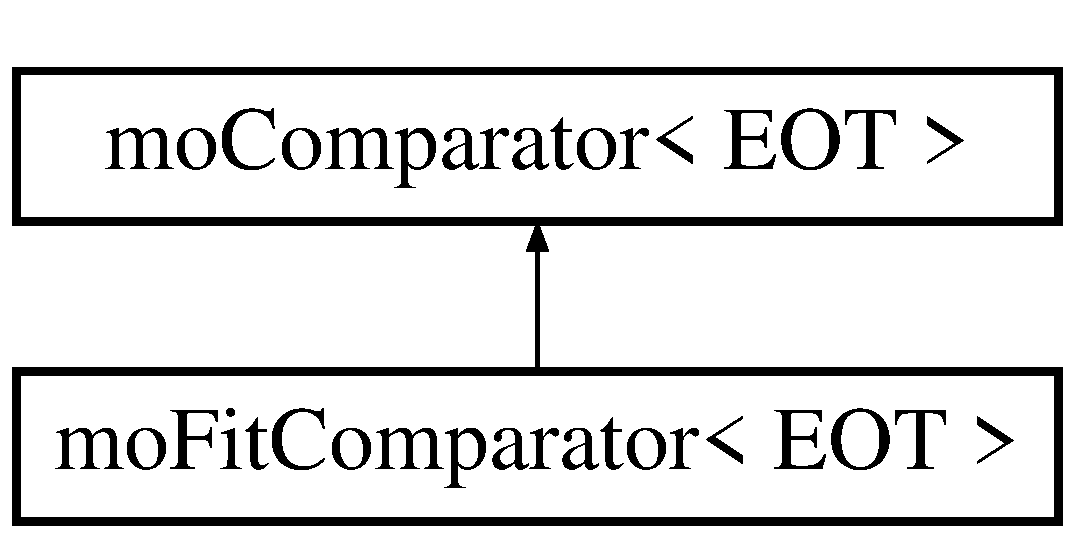
\includegraphics[height=4cm]{classmo_fit_comparator}
\end{center}
\end{figure}
\subsection*{Public Member Functions}
\begin{CompactItemize}
\item 
bool {\bf operator()} (const EOT \&\_\-solution1, const EOT \&\_\-solution2)
\begin{CompactList}\small\item\em Function which makes the comparison and gives the result. \item\end{CompactList}\end{CompactItemize}


\subsection{Detailed Description}
\subsubsection*{template$<$class EOT$>$ class mo\-Fit\-Comparator$<$ EOT $>$}

Comparison according to the fitness. 

An EOT is better than an other if its fitness is better. 



Definition at line 46 of file mo\-Fit\-Comparator.h.

\subsection{Member Function Documentation}
\index{moFitComparator@{mo\-Fit\-Comparator}!operator()@{operator()}}
\index{operator()@{operator()}!moFitComparator@{mo\-Fit\-Comparator}}
\subsubsection{\setlength{\rightskip}{0pt plus 5cm}template$<$class EOT$>$ bool {\bf mo\-Fit\-Comparator}$<$ EOT $>$::operator() (const EOT \& {\em \_\-solution1}, const EOT \& {\em \_\-solution2})\hspace{0.3cm}{\tt  [inline, virtual]}}\label{classmo_fit_comparator_a0}


Function which makes the comparison and gives the result. 

\begin{Desc}
\item[Parameters:]
\begin{description}
\item[{\em \_\-solution1}]The first solution. \item[{\em \_\-solution2}]The second solution. \end{description}
\end{Desc}
\begin{Desc}
\item[Returns:]true if the fitness of the first solution is better than the second solution, false else. \end{Desc}


Implements {\bf eo\-BF$<$ const EOT \&, const EOT \&, bool $>$}.

Definition at line 56 of file mo\-Fit\-Comparator.h.

The documentation for this class was generated from the following file:\begin{CompactItemize}
\item 
mo\-Fit\-Comparator.h\end{CompactItemize}
